\documentclass[a4,10pt,zihao=-4]{ctexart}
\linespread{1.0} % 设置单倍行距

\usepackage{ctex}
\usepackage[utf8]{inputenc}
\usepackage{amsfonts,amsmath,amscd,amssymb,amsthm}
\usepackage{latexsym,bm}
\usepackage{cite}
\usepackage{mathtools,mathdots,graphicx,array}
\usepackage{fancyhdr}
\usepackage{lastpage}
\usepackage{color}
\usepackage{enumitem}
\usepackage{mpdoc}
\usepackage{diagbox}
\usepackage{xcolor,tcolorbox,tikz,tkz-tab,mdframed,tikz-cd}
\usepackage{framed}
\usepackage{verbatim}
\usepackage{extarrows}
\usepackage{fontspec}
\graphicspath{{./assets/}}  % 设置图片的默认路径

\begin{document}
\pagenumbering{roman}
\title{实验三\,\,\,\,芯片的封装与应用}

\author{李雨轩 2204112913 计算机2205}
\date{2024年6月}
\maketitle

\section{实验目的}
\begin{enumerate}
  \item 掌握Verilog语言框架,编程及调试的方法。
  \item 熟悉Verilog的基本语法。
  \item 掌握Vivado开发平台及FPGA开发板的使用。
\end{enumerate}

\section{实验内容}
\begin{enumerate}   
  \item 完成74LS161计数器芯片的实现、测试及6进制计数器的实现,将程序下载到FPGA开发板进行验证。
  \item 分析电路中的竞争与冒险,给出解决方案。
  \item 将芯片及相关模块封装为IP核,通过原理图设计实现N进制计数器,记录、分析仿真波形和电路图。
\end{enumerate}

\section{实验要求}
\begin{enumerate}
  \item 说明电路功能,分析设计、仿真代码和电路图。
  \item 分析仿真波形,观察输入输出是否与预期电路功能相符(测试要全面,关注特殊情况的测试)。
  \item 记录设计和调试过程。
\end{enumerate}


\newpage
\section{实验过程及结果分析}
\subsection{6进制计数器的设计}

\subsubsection{74LS161芯片}

\paragraph{1. 设计文件及仿真文件}:

\vspace{1em}
\noindent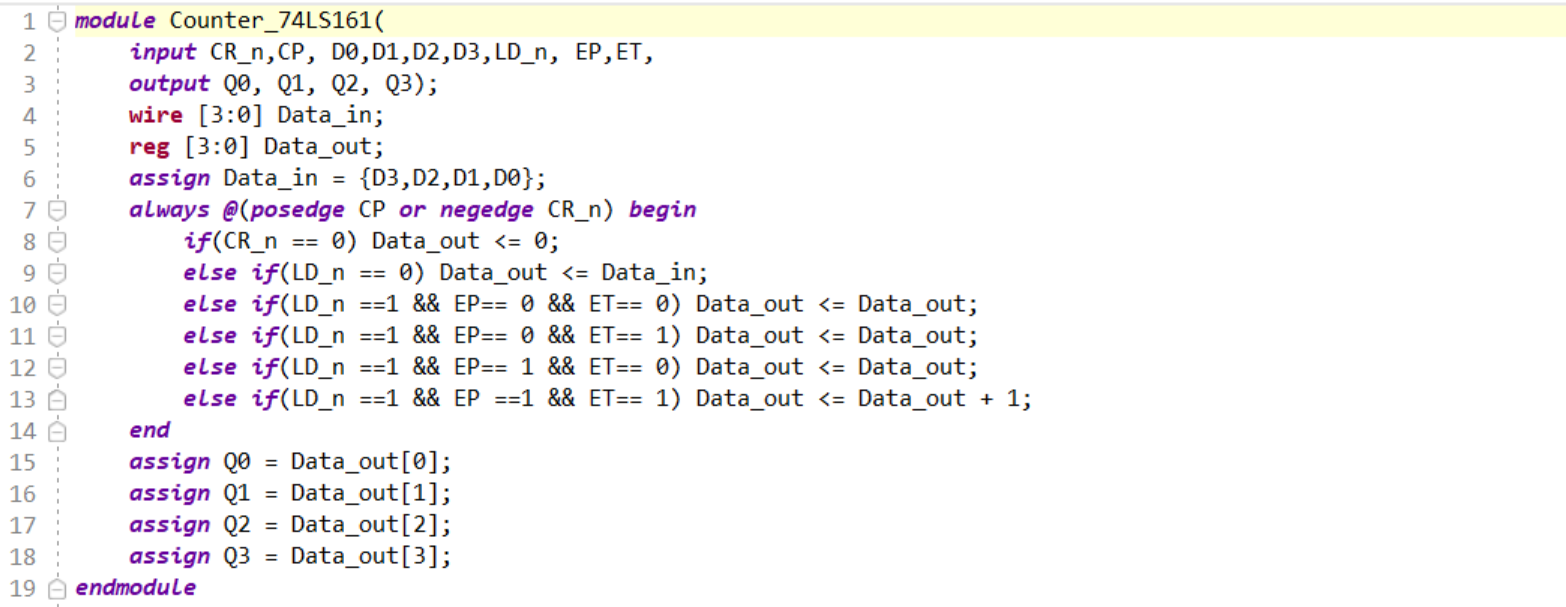
\includegraphics[width=1\textwidth]{Counter_74LS161_code.png}

模块 Counter\_74LS161 模拟了使用74LS161同步计数器IC实现的4位计数器功能。它接收多个输入信号,包括时钟 (CP)、异步复位 (CR\_n)、数据输入 (D0 到 D3)、加载使能 (LD\_n) 和控制信号 (EP, ET)。 Data\_in 信号由输入数据线派生而来。

always 块在时钟上升沿 (CP) 或复位下降沿 (CR\_n) 触发。根据控制信号 (LD\_n, EP, ET),它更新 Data\_out 寄存器:如果复位 (CR\_n) 激活,则将 Data\_out 复位为0;如果加载使能 (LD\_n) 激活,则使用 Data\_in 加载 Data\_out;根据 EP 和 ET 的组合,保持 Data\_out 或将其增加1。

该模块输出存储在 Data\_out 中的4位计数值 (Q0 到 Q3),供外部使用。


模块 Counter\_74LS161 的仿真文件如下:

\vspace{1em}
\noindent\includegraphics[width=1\textwidth]{sim_74LS161_code.png}

\paragraph{2. RTL分析及仿真结果:}

通过RTL分析生成如下Schematic,并使用上述仿真文件验证模块 Counter\_74LS161的正确性。

\vspace{1em}
\noindent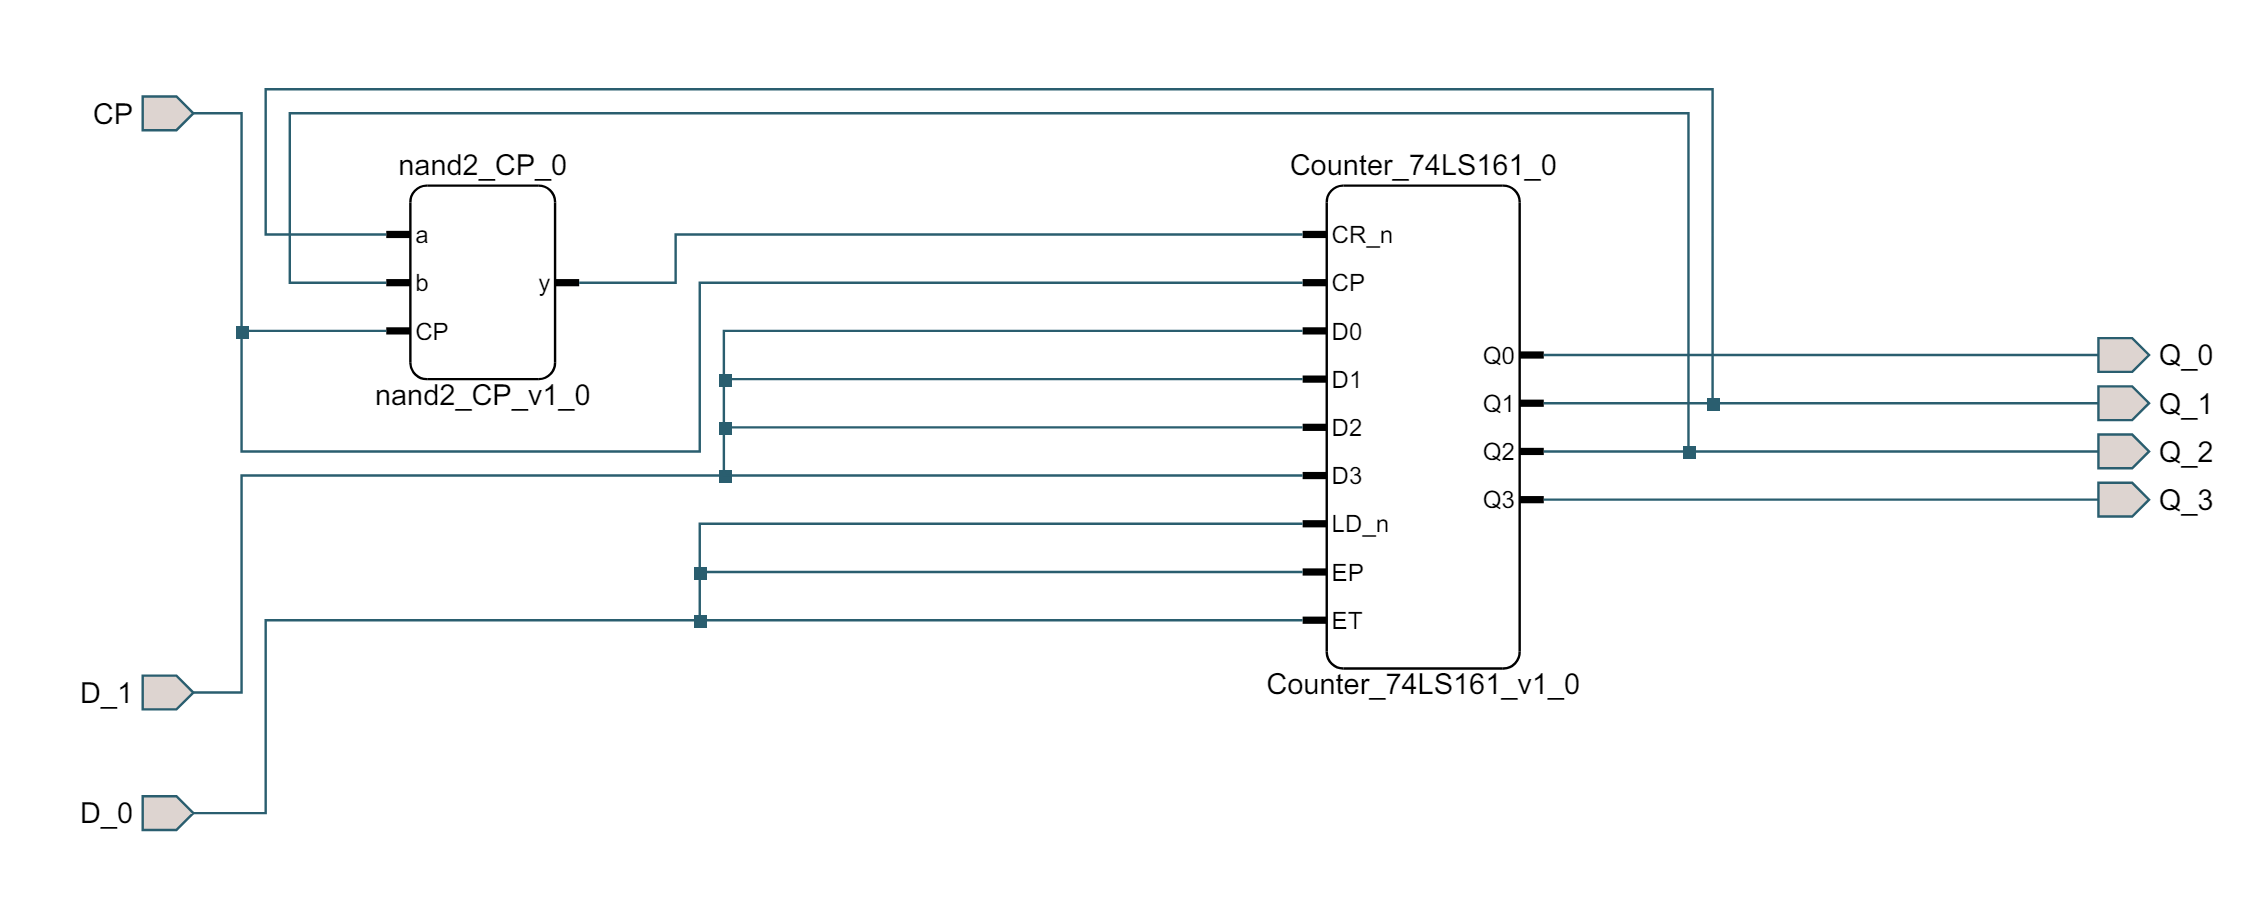
\includegraphics[width=0.7\textwidth]{Counter_74LS161_pic.png}

\noindent\includegraphics[width=1\textwidth]{sim_74LS161_sim.png}



\subsubsection{时钟分频及EGo1数码管显示模块}

\vspace{1em}
\noindent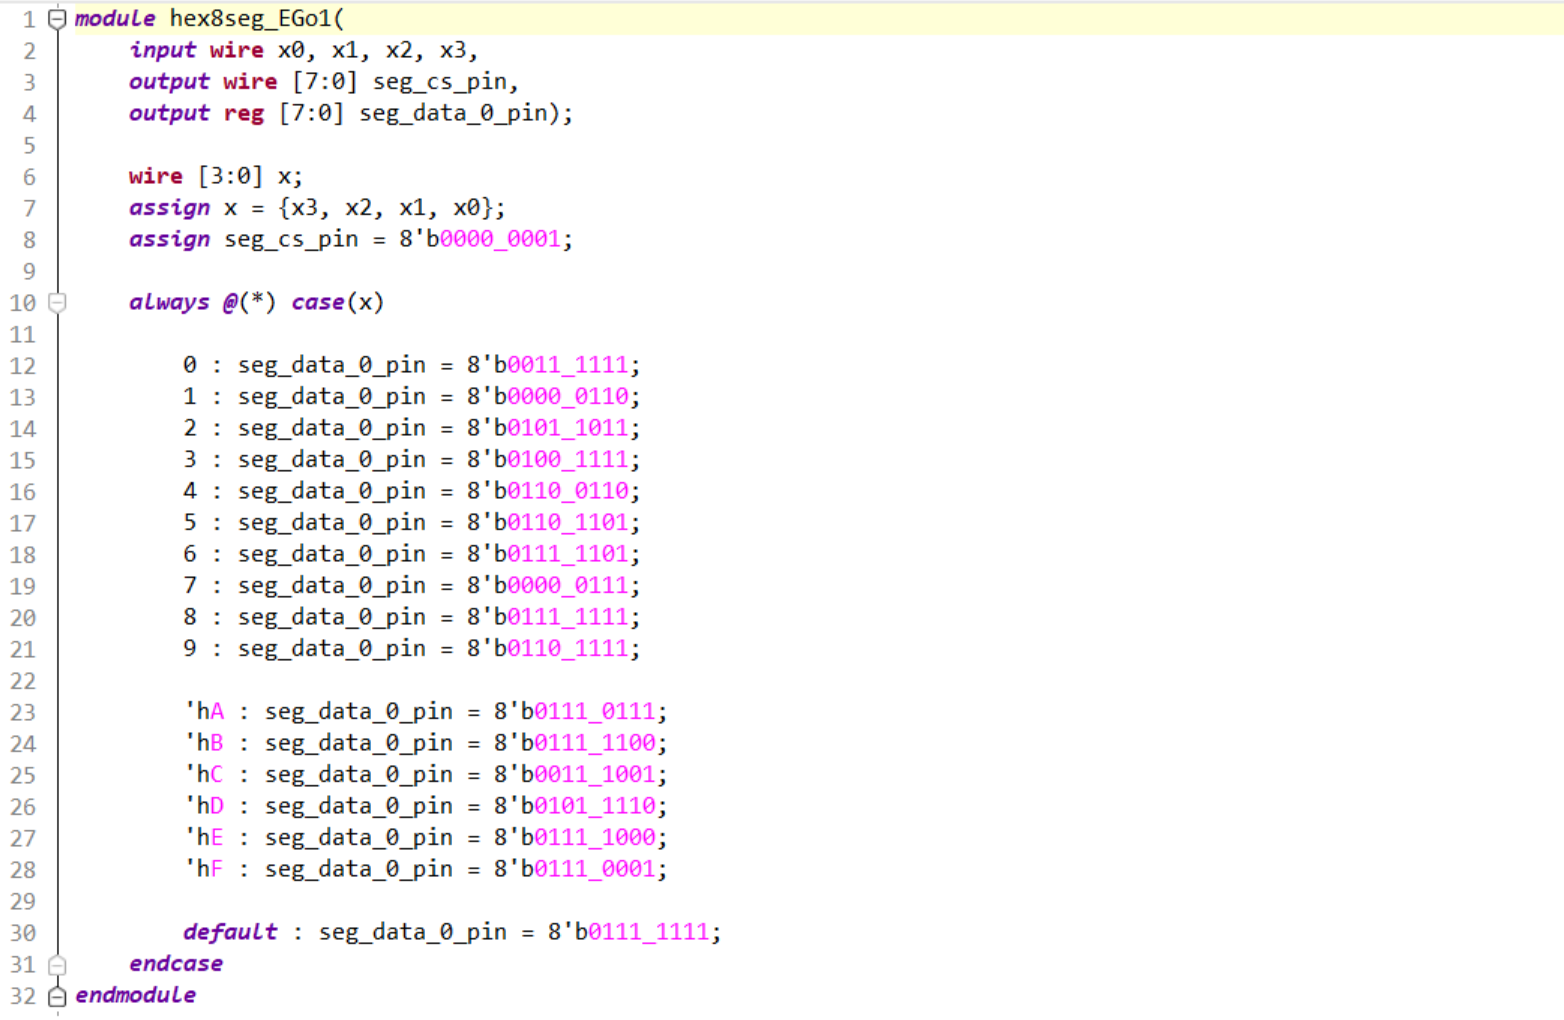
\includegraphics[width=1\textwidth]{hex8seg_EGo1_code.png}

模块 \texttt{hex8seg\textunderscore EGo1} 实现了一个将四位输入信号转换为七段数码管显示的功能。根据输入信号 \texttt{x0} 到 \texttt{x3} 组成的四位数,通过组合逻辑将其转换为对应的七段数码管显示数据。模块中定义了 \texttt{seg\textunderscore cs\textunderscore pin} 和 \texttt{seg\textunderscore data\textunderscore 0\textunderscore pin} 作为输出端口,其中 \texttt{seg\textunderscore cs\textunderscore pin} 被赋值为固定的 8 位二进制数 \texttt{0000\textunderscore 0001},用于控制数码管选通信号。\texttt{seg\textunderscore data\textunderscore 0\textunderscore pin} 则根据输入信号 \texttt{x} 的不同取值,使用 \texttt{case} 语句来分别设置为对应的七段数码管数据值。如果输入的 \texttt{x} 值不在定义的范围内(0 到 9 和 A 到 F),则默认将 \texttt{seg\textunderscore data\textunderscore 0\textunderscore pin} 设置为全灭状态 \texttt{0111\textunderscore 1111},即数码管不显示任何内容。

\vspace{1em}
\noindent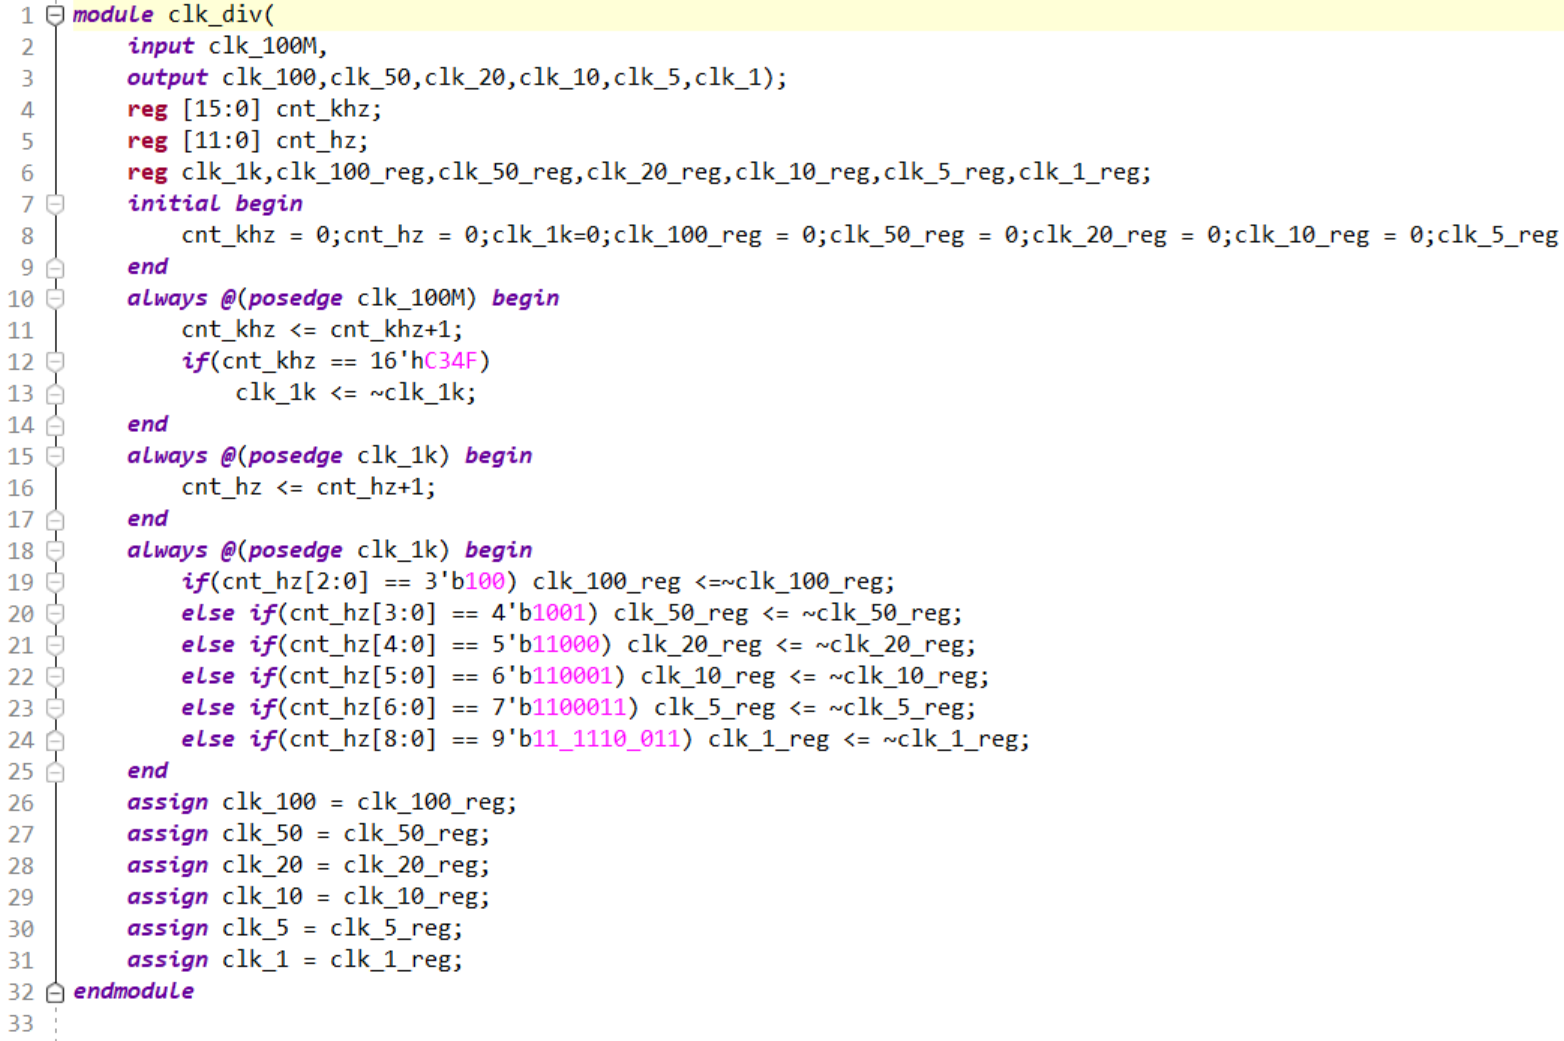
\includegraphics[width=1\textwidth]{clk_div_code.png}

模块 `clk\_div` 实现了一个时钟分频器,将输入的100MHz时钟信号 `clk\_100M` 分频为多个不同频率的时钟信号输出。模块中使用了多个计数器 `cnt\_khz` 和 `cnt\_hz` 来实现不同的分频比例。具体而言,`cnt\_khz` 计数到 16'hC34F(49999)时,产生1kHz的时钟信号 `clk\_1k`,作为进一步分频的基准。随后,`cnt\_hz` 计数的结果用于分别控制生成的时钟信号 `clk\_100`、`clk\_50`、`clk\_20`、`clk\_10`、`clk\_5`、`clk\_1` 的频率。这些时钟信号根据不同的计数条件在相应的 `always` 块内被翻转和赋值,最终通过 `assign` 语句输出到模块的端口上,供外部电路使用。



\subsubsection{基于EGo1开发板的6进制计数器}

\vspace{1em}
\noindent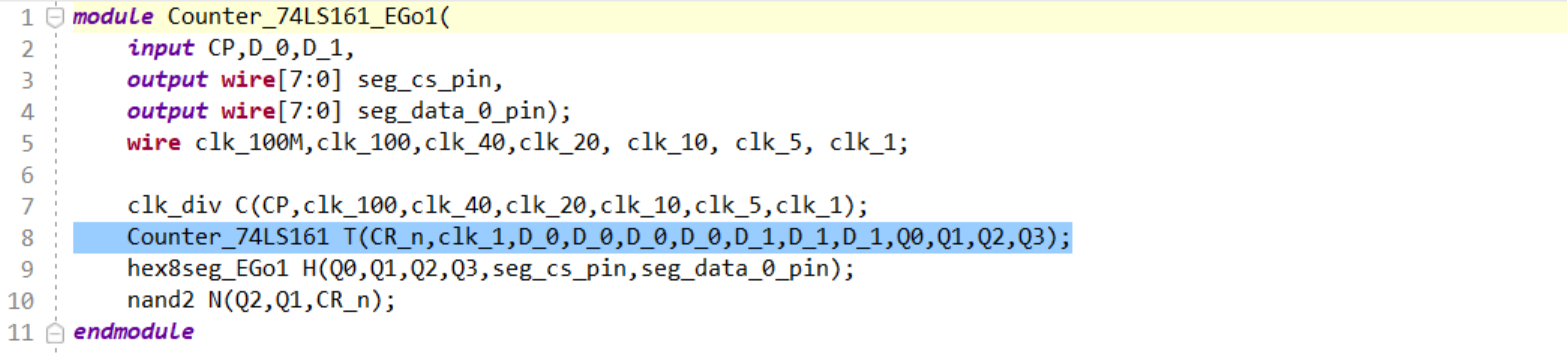
\includegraphics[width=1\textwidth]{assets/Counter_74LS161_EGo1_nand2_code.png}

模块 \texttt{Counter\_74LS161\_EGo1} 组合了多个子模块,实现了一个综合性的数字电路功能。模块中包含了输入时钟信号 \texttt{CP} 和数据输入信号 \texttt{D\_0}、\texttt{D\_1},以及输出的七段数码管控制信号 \texttt{seg\_cs\_pin} 和数据信号 \texttt{seg\_data\_0\_pin}。在内部,它实例化了以下几个模块:首先是 \texttt{clk\_div} 模块,用来分频输入时钟信号 \texttt{CP},并产生多个分频后的时钟信号 \texttt{clk\_100}、\texttt{clk\_40}、\texttt{clk\_20}、\texttt{clk\_10}、\texttt{clk\_5}、\texttt{clk\_1};接着是 \texttt{Counter\_74LS161} 模块 \texttt{T},用来计数并输出四位计数值 \texttt{Q0}、\texttt{Q1}、\texttt{Q2}、\texttt{Q3};然后是 \texttt{hex8seg\_EGo1} 模块 \texttt{H},将四位计数值转换为七段数码管显示的控制信号;最后是 \texttt{nand2\_CP} 模块 \texttt{N},它使用 \texttt{Q2} 和 \texttt{Q1} 的值来控制异步复位信号 \texttt{CR\_n}。

通过这样的组合,\texttt{Counter\_74LS161\_EGo1} 模块实现了从时钟分频、计数、数码管显示到复位控制的完整功能,每个子模块分别负责其特定的任务,最终合并在一起实现复杂的数字逻辑功能。

同时还需要如下的配置文件:

\vspace{1em}
\noindent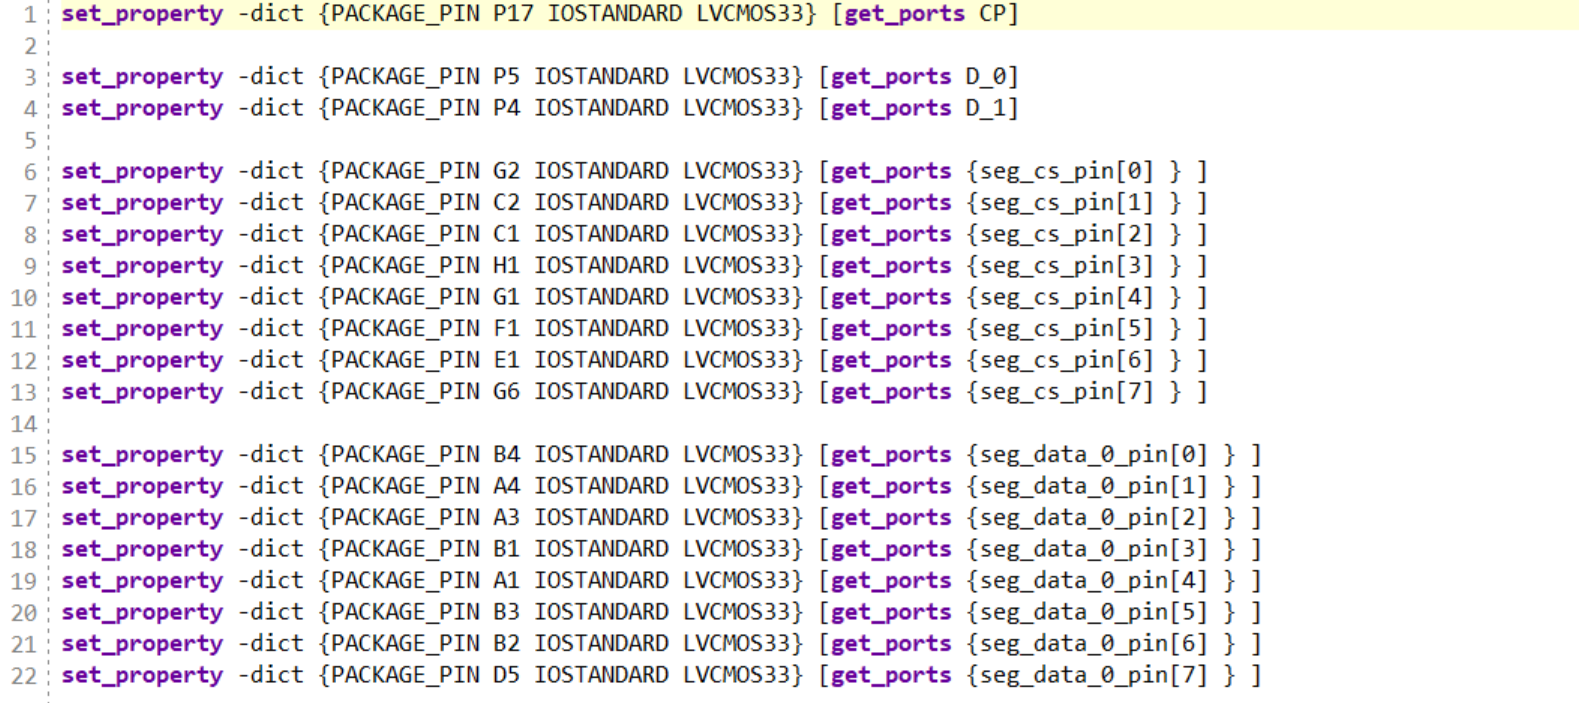
\includegraphics[width=1\textwidth]{assets/contin_code.png}

\subsubsection{将带时钟分频和数码管显示的6进制计数器烧录到开发板进行验证}

RTL分析、SIMULATION仿真分析验证功能实现无误后,通过SYNTHESIS、IMPLEMENTATION、Generate Bitstream以及Program Device步骤,成功在EGo1开发板上实现计数器功能。但是发现实际运行时EGo1开发板上实现的是一个四进制的计数器,原因在于不同路径输入信号变化传输到同一点门级电路,时间上有先后,也就是存在竞争现象导致冒险产生了错误输出,如下图展示的那样

\vspace{1em}
\noindent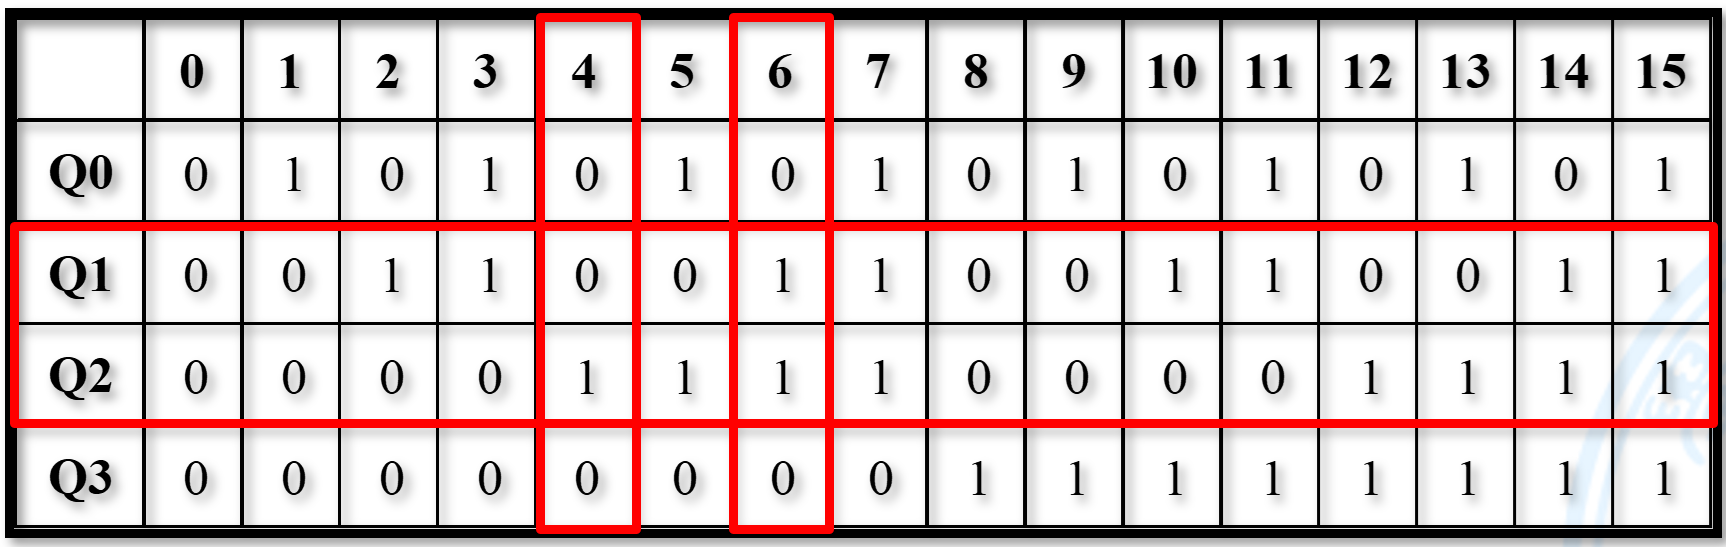
\includegraphics[width=1\textwidth]{assets/table1.png}
\noindent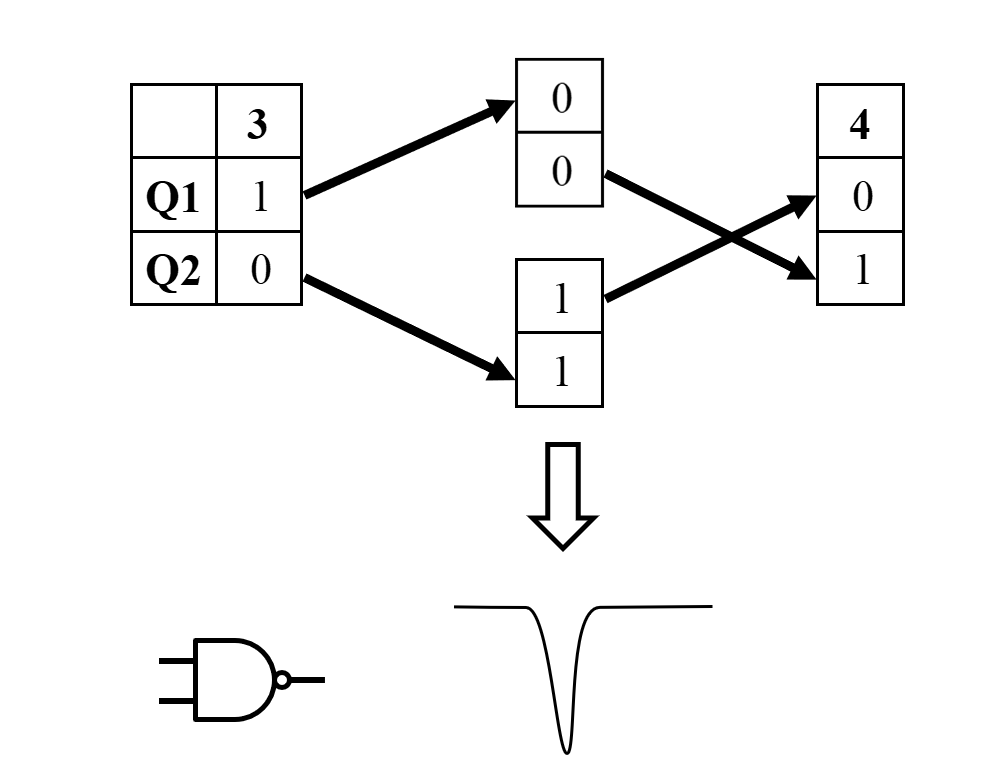
\includegraphics[width=1\textwidth]{assets/table2.png}

因此修改nand2模块如下,同时将模块 \texttt{Counter\_74LS161\_EGo1} 中对于nand2的调用修改为\texttt{nand2\_CP N(Q2,Q1,CR\_n);}

\vspace{1em}
\noindent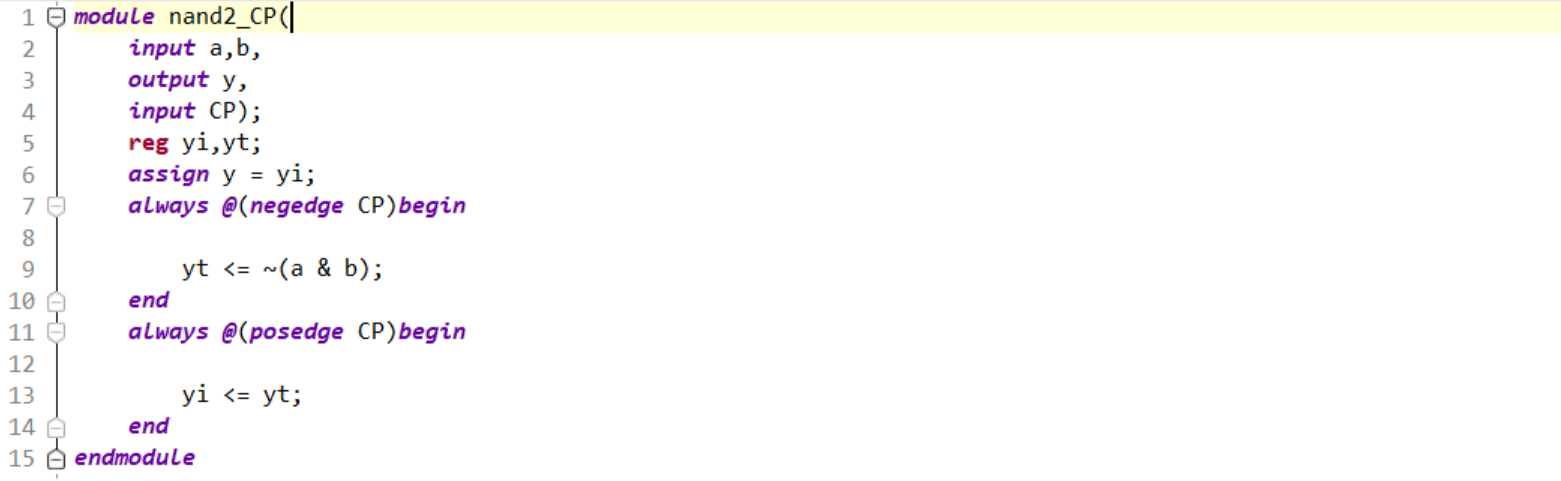
\includegraphics[width=1\textwidth]{assets/nand2_CP_code.png}

模块 nand2\_CP 实现了一个带有时钟控制的NAND门。它的设计思路是利用两个时钟边沿敏感的触发器(always块),一个在时钟下降沿触发,另一个在时钟上升沿触发。这种设计与普通的NAND门不同之处在于,它确保了输出y在时钟信号CP的稳定时刻更新,避免了在输入变化时输出y不稳定的情况发生。这种时钟控制的NAND门适用于需要同步输入和输出的电路设计,保证了在时钟信号的不同相位上,输入信号的变化不会导致竞争条件的出现,确保了信号在时序上的正确性和稳定性。

修改后再次由RTL分析、SIMULATION仿真分析验证功能实现无误后,通过SYNTHESIS、IMPLEMENTATION、Generate Bitstream以及Program Device步骤,成功在EGo1开发板上实现计数器功能。如下图所示:

\vspace{1em}
\noindent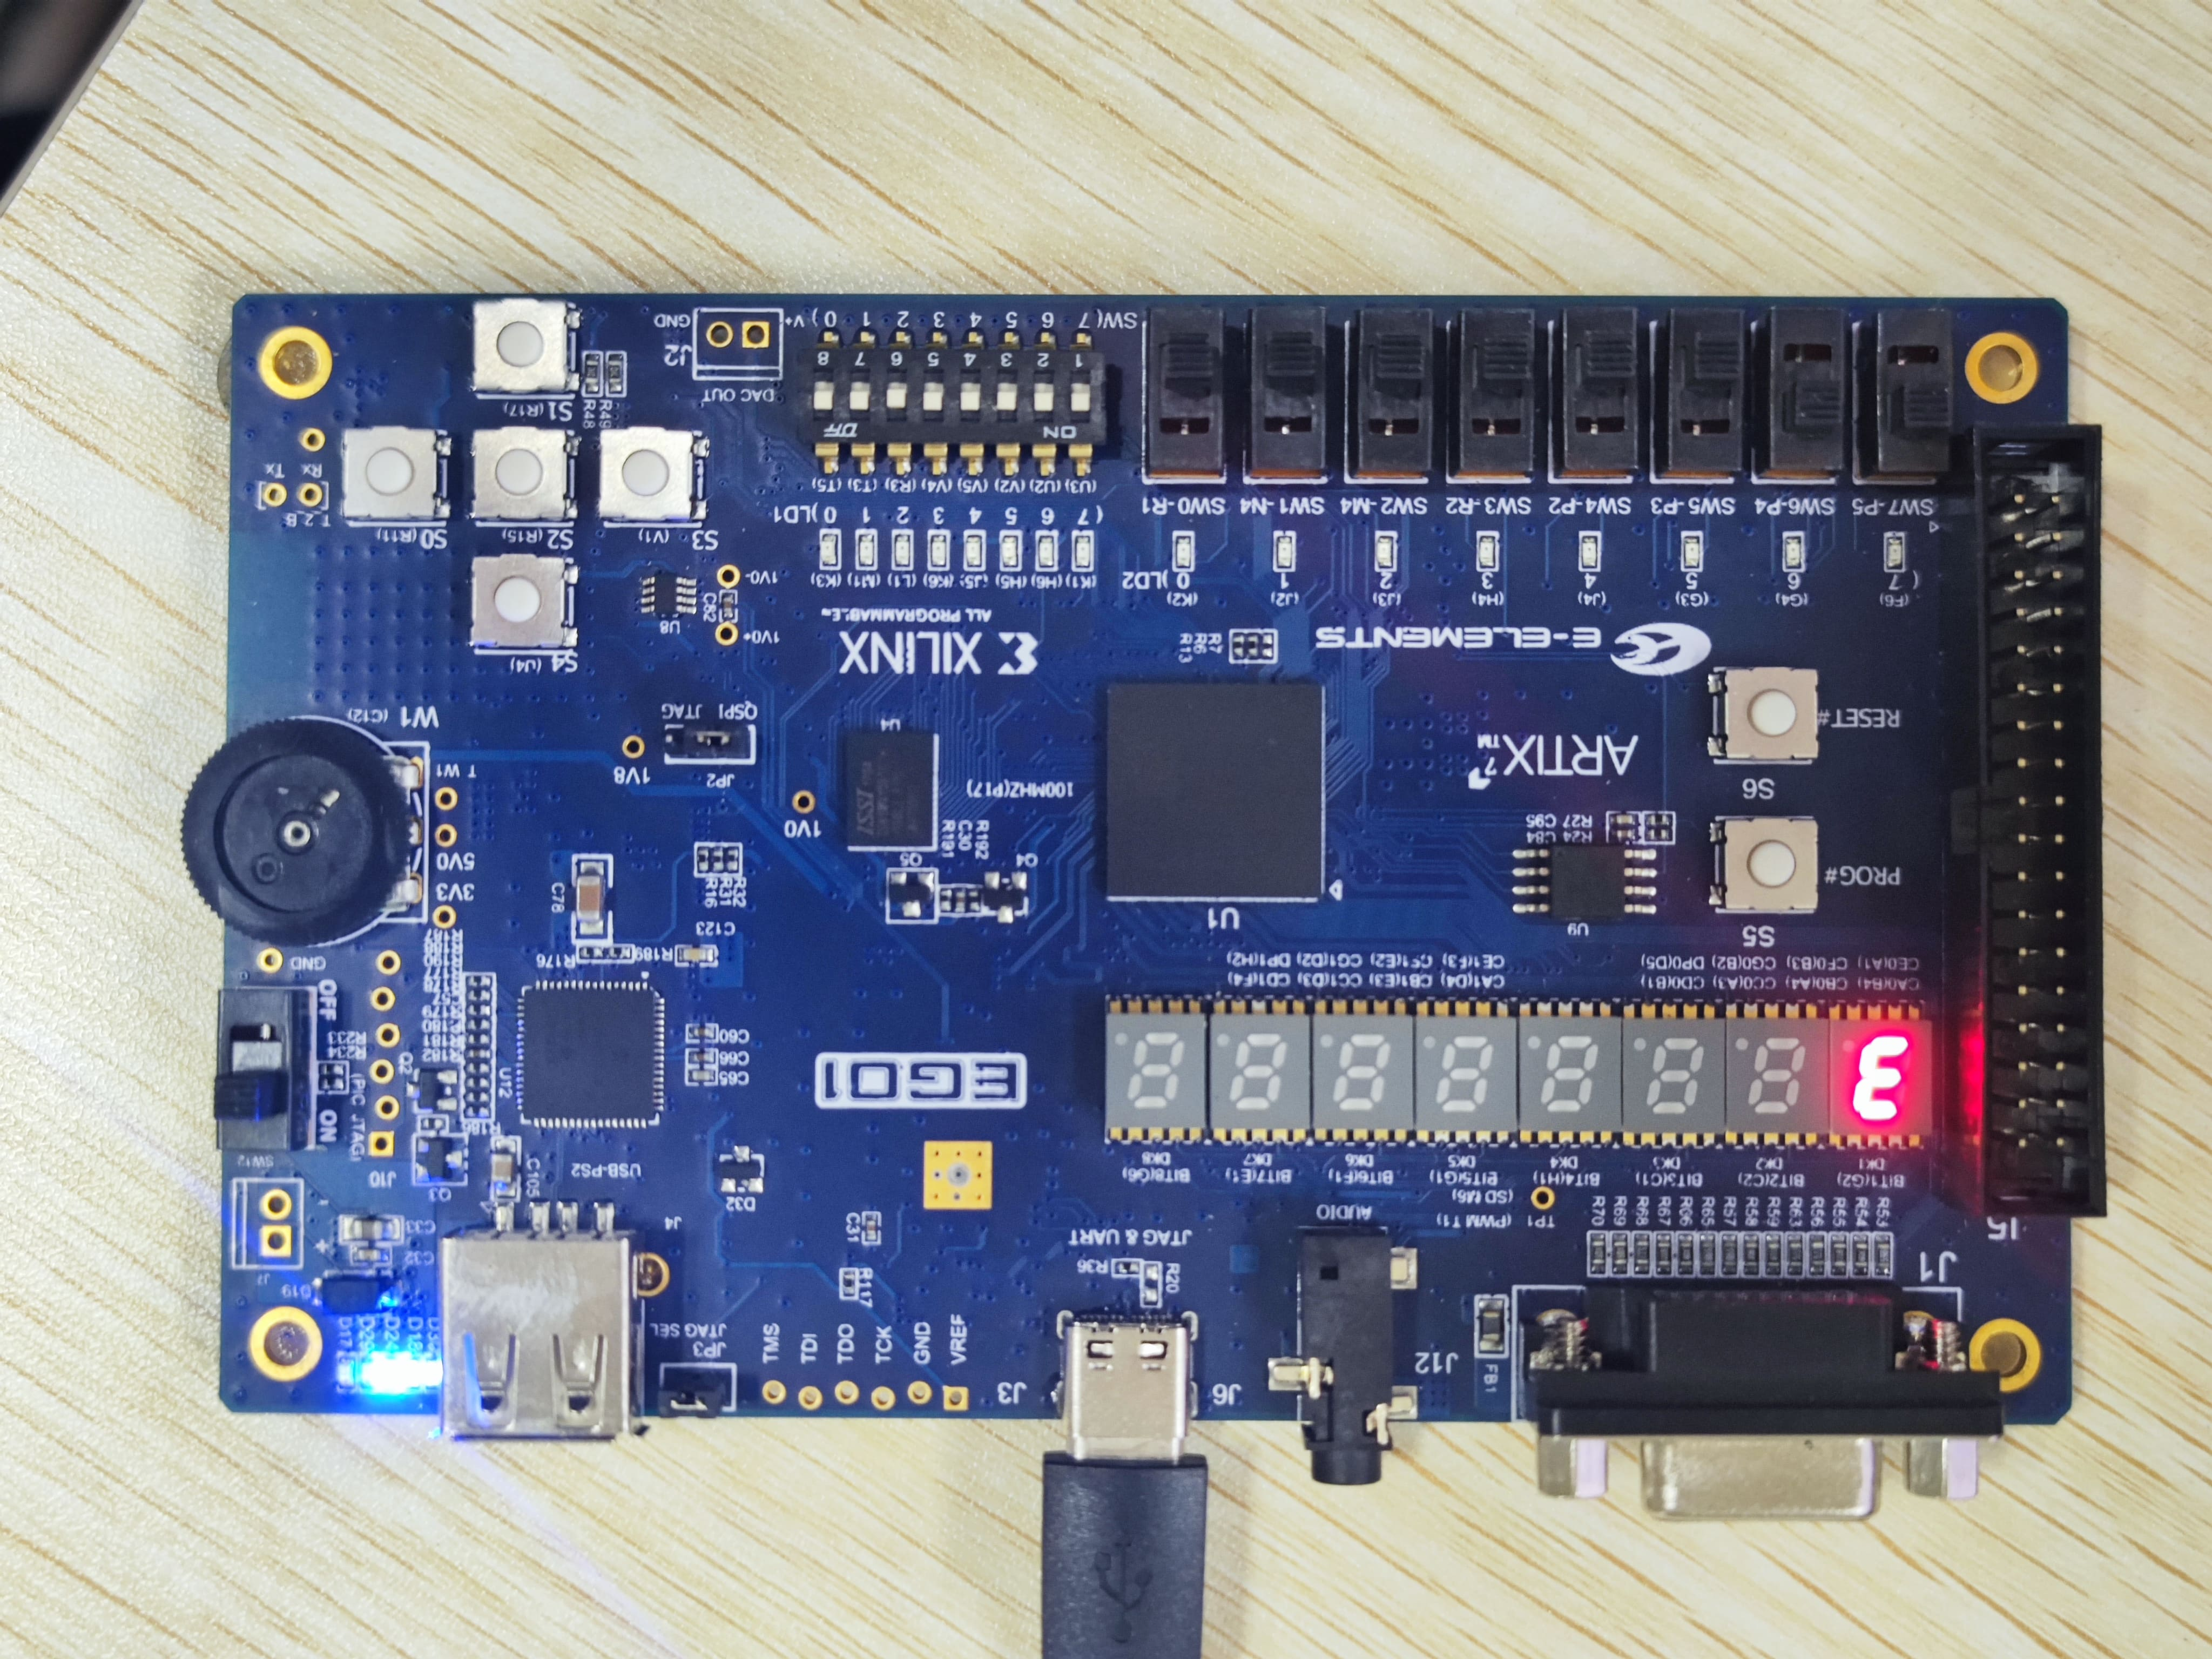
\includegraphics[width=0.8\textwidth]{assets/ego1.jpg}


\subsection{原理图设计13进制计数器(0-12)}

由于开发板验证电路正确后,可以将各子模块封装为IP,采用原理图设计方式实现N进制计数器,每个模块单独工程封装。

所以在完成对二输入与非门 ( nand2 ) 模块和71LS161芯片模块的IP封装后,在原理图设计-新建工程-设置-添加IP目录后,本人采用原理图设计实现一个13进制计数器(学号后两位)

通过鼠标拖动连接各模块接口连线;选中输入/输出端口,右键选择“Create Port/Make External”创建输入输出接口。

下面是13进制计数器原理图:

\vspace{1em}
\noindent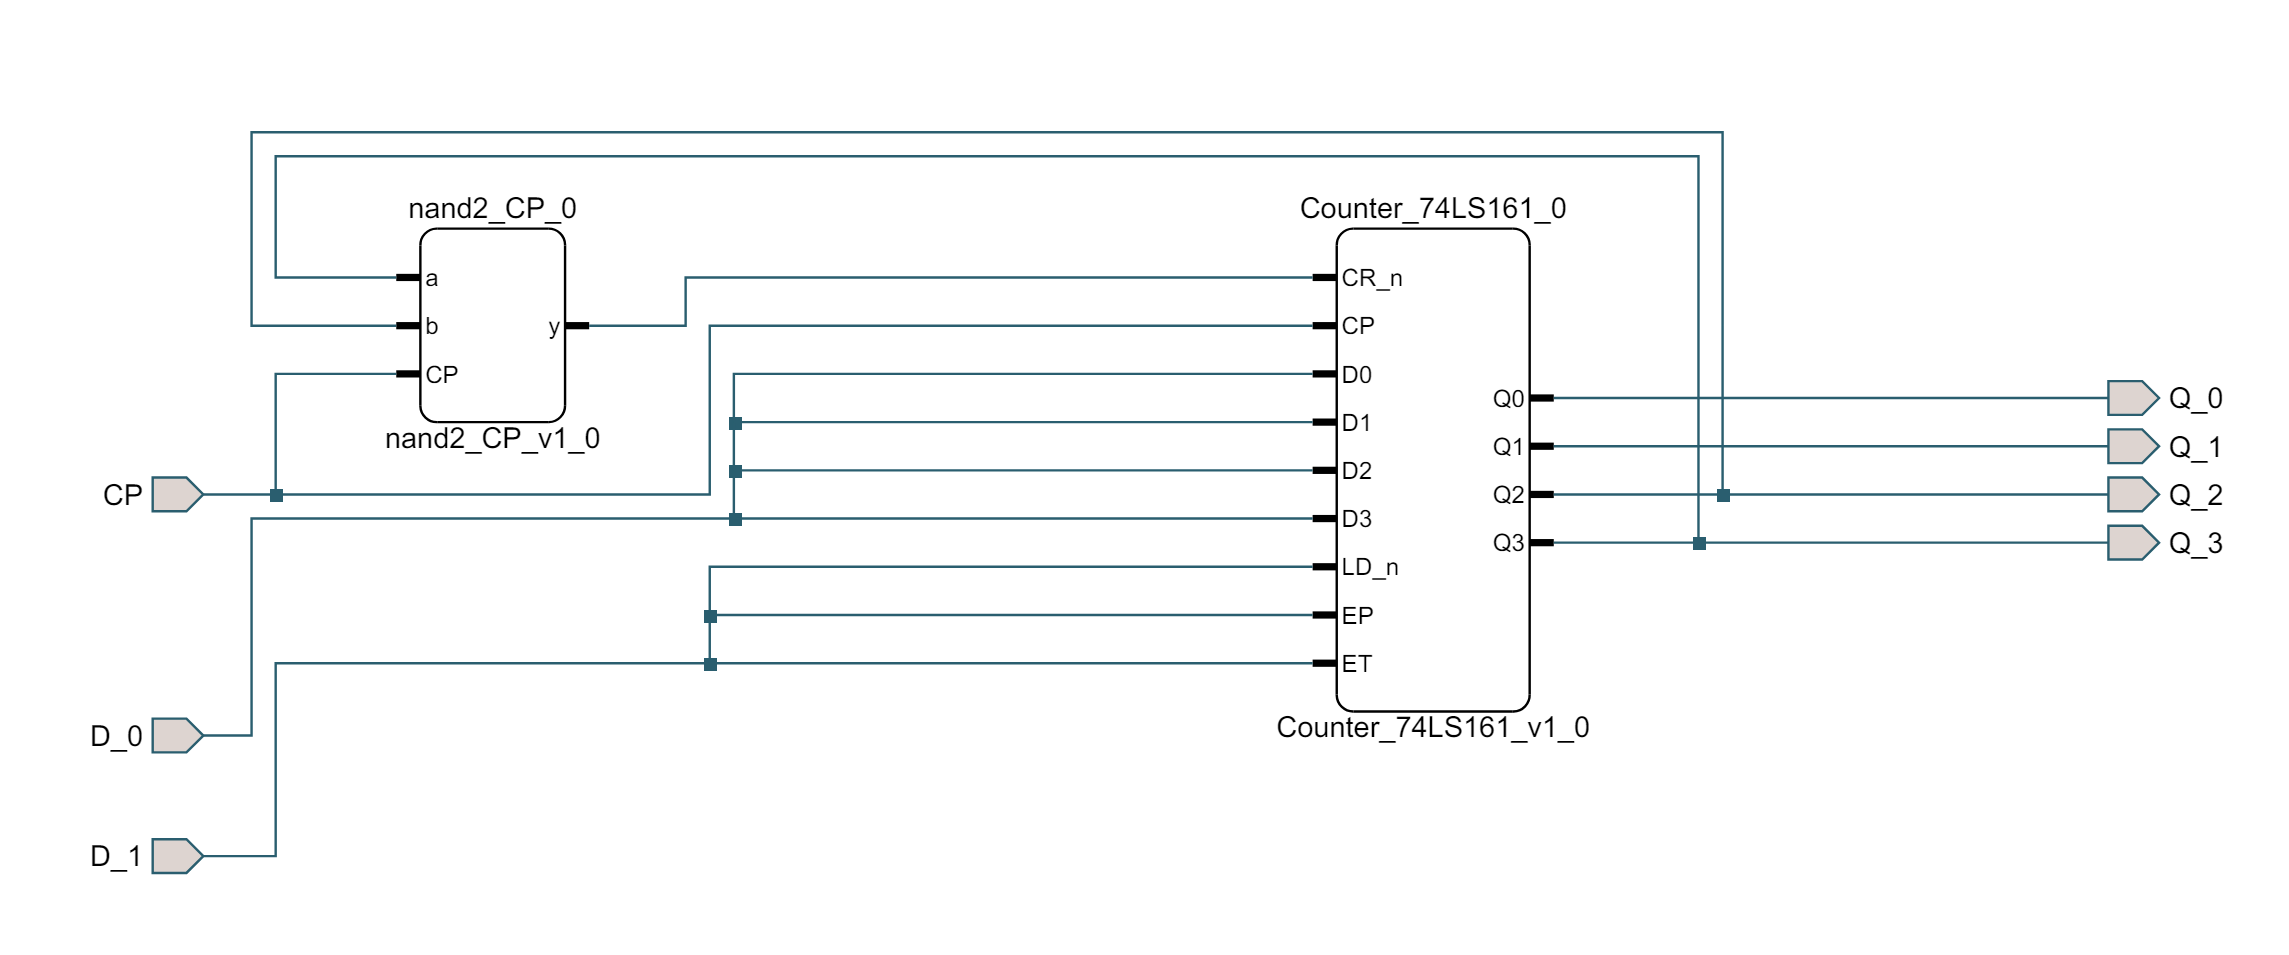
\includegraphics[width=1\textwidth]{assets/12c.png}

实现的逻辑就是将计数值为12时作为起跳状态,检测到2时向同步置零信号发送1,这样下一时刻就会进入0。

同时编写仿真文件,产生波形图如下:

\vspace{1em}
\noindent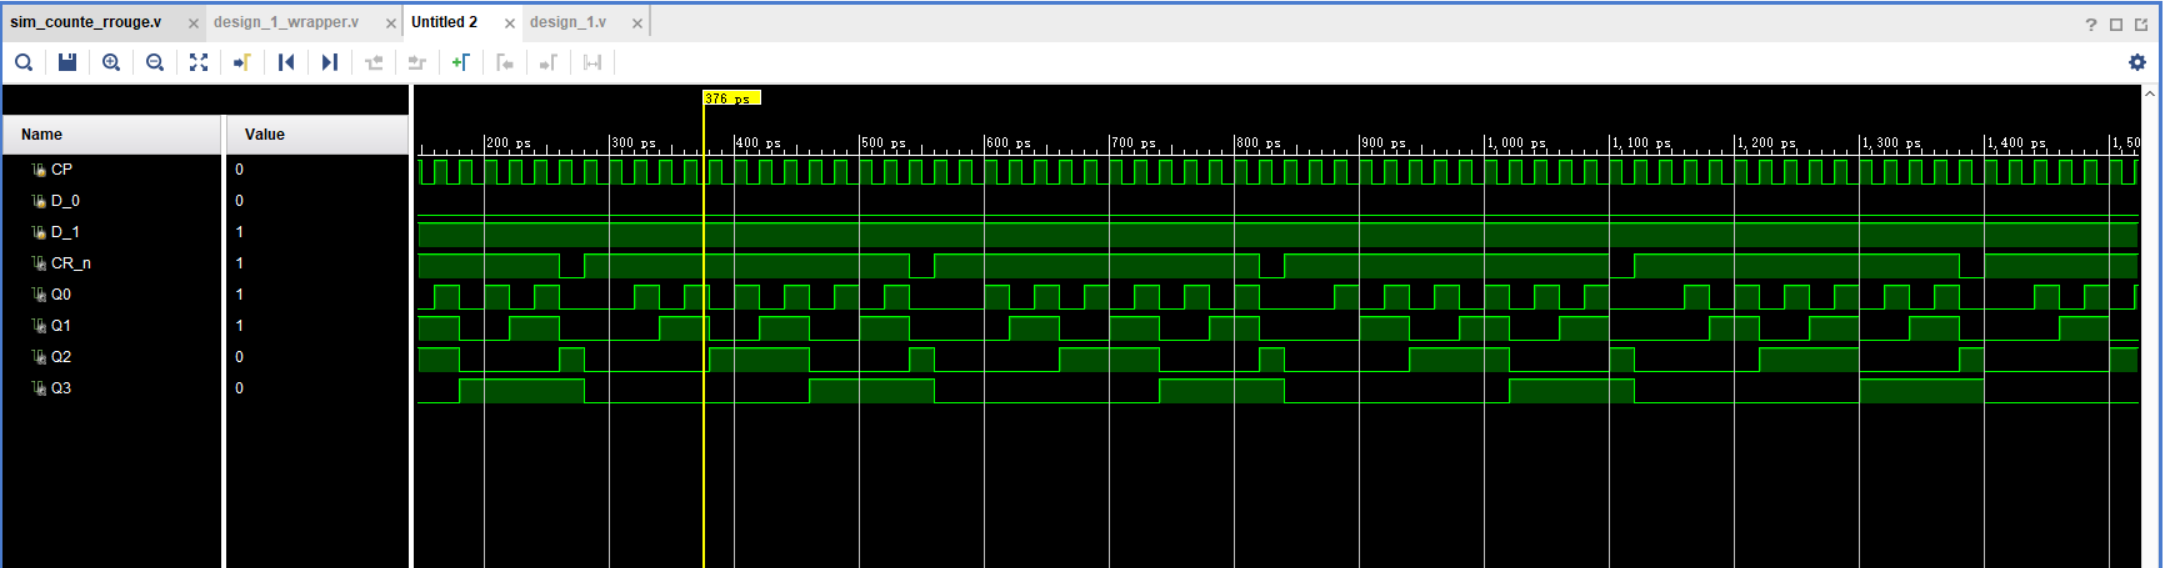
\includegraphics[width=1\textwidth]{assets/counter13_sim.png}



\section{思考题: 如何利用多片74LS161芯片实现如24进制计数器}
为实现模24的计数器(计数范围从00000到10111),通过级联多个74LS161芯片来实现所需的计数范围。在这之前要为74LS161芯片添加进位输出 (RCO) 。

\subsection{设计思路}
需要计数从0到23(十进制),即从00000到10111(二进制)。对于这个一个5位二进制计数器,可以分解为两个部分:
\begin{itemize}
  \item 一个4位计数器,实现低4位的计数。
  \item 一个2位计数器,实现高1位的计数。
\end{itemize}

具体来说,我们可以用以下方式实现:
\begin{enumerate}
  \item 使用两个74LS161芯片级联来实现5位计数器。
  \item 第一个74LS161芯片(低位计数器)计数从0000到1111。
  \item 第二个74LS161芯片(高位计数器)实现对低位计数器的溢出计数,即在低位计数器从1111变为0000时,高位计数器计数加1。
\end{enumerate}

\subsection{具体电路连接}

\subsubsection{低位计数器(74LS161\_1)}
\begin{itemize}
  \item 时钟输入 (CP) 接系统时钟。
  \item 异步清零 (CR\_n) 接地(低电平有效)。
  \item 使能输入 (ET 和 EP) 接高电平。
  \item 进位输出 (RCO) 连接到高位计数器的使能输入 (ET)。
  \item 数据输入 (D0-D3) 接地。
  \item 加载使能 (LD\_n) 接高电平。
\end{itemize}

\subsubsection{高位计数器(74LS161\_2)}
\begin{itemize}
  \item 时钟输入 (CP) 接低位计数器的进位输出 (RCO)。
  \item 异步清零 (CR\_n) 接地(低电平有效)。
  \item 使能输入 (EP) 接高电平,(ET) 接低位计数器的进位输出 (RCO)。
  \item 数据输入 (D0-D3) 仅需要D0和D1,接地。
  \item 加载使能 (LD\_n) 接高电平。
\end{itemize}

\subsubsection{实现模24的逻辑}
\begin{itemize}
  \item 高位计数器的输出Q1和Q0以及低位计数器的输出Q3和Q2构成5位计数器的前5位。
  \item 当计数值达到24(11000)时,需要复位两个计数器。
  \item 可以通过组合逻辑来检测高位计数器输出Q1为1、Q0为0、低位计数器Q3为1和Q2为0,并通过一个与门控制两个计数器的CR\_n输入。
\end{itemize}

\subsection{verilog代码实现}

\begin{verbatim}
module mod24_counter (
    input wire clk,
    input wire reset,
    output wire [4:0] count
);
    wire [3:0] low_count;
    wire [1:0] high_count;
    wire rco_low, reset_all;
    
    // 低位计数器
    Counter_74LS161 low_counter (
        .CP(clk),
        .CR_n(reset_all),
        .EP(1'b1),
        .ET(1'b1),
        .LOAD(1'b1),
        .D(4'b0000),
        .Q(low_count),
        .RCO(rco_low)
    );
    
    // 高位计数器
    Counter_74LS161 high_counter (
        .CP(rco_low),
        .CR_n(reset_all),
        .EP(1'b1),
        .ET(rco_low),
        .LOAD(1'b1),
        .D(4'b0000),
        .Q({2'b00, high_count}),
        .RCO()
    );
    
    // 检测模24的复位逻辑
    assign reset_all = reset | (high_count == 2'b10 && low_count[3:2] == 2'b11);
    assign count = {high_count, low_count};
    
endmodule
\end{verbatim}


通过上述步骤,可以成功实现一个模24的计数器。


\section{调试和心得体会}

\subsection{调试过程}

在初步在EGo1开发板上验证时,发现实际运行时计数器显示的是一个四进制计数器,而不是预期的六进制计数器。经过仔细观察和分析,发现是由于竞争和冒险现象导致了错误的计数输出。所以我进行了如下的调试过程:

\begin{itemize}
    \item 修改NAND门模块的Verilog代码,增加时钟控制逻辑,确保同步更新输出。
    
    \item 使用RTL分析和仿真工具验证修改后的功能正确性。

    \item 重新生成Bitstream并在EGo1开发板上烧录,验证计数器功能成功按预期工作
    
\end{itemize}


\subsection{心得体会}


在本次实验中,我深入理解了Verilog语言的基本语法和模块化设计原则。通过对74LS161计数器芯片的实现,我不仅学会了如何编写和调试Verilog代码,还掌握了如何利用仿真工具验证电路功能的正确性。

通过本次实验,我也意识到了实验设计和文档记录的重要性。详细的实验设计和清晰的文档记录帮助我更好地理解和复习实验内容,确保了实验的顺利进行和成果的有效展示。

在今后的学习和工作中,我将继续深入学习数字电路设计和FPGA开发技术,不断提升自己的实践能力和解决问题的能力。通过更多实验和项目,我希望能够在硬件设计领域取得更多的学习。


\end{document}
